% vim: set foldmethod=marker foldlevel=0:

\documentclass[a4paper]{article}
\usepackage[UKenglish]{babel}

\usepackage{preamble}

\usepackage{graphicx}
\graphicspath{ {./imgs/} }

\fancyhead[L]{MA139 Assignment 2}
\title{MA139 Analysis 2, Assignment 2}
\colorlet{questionbodycolor}{cyan!50}

\begin{document}

\maketitle

\setlength{\parindent}{0em}
\setlength{\parskip}{1em}

% {{{ Q1
\question{1}

\begin{questionbody}
Let $(x_i)_1^n$ be a finite sequence of positive numbers whose mean is \[
m = \f1n \sum_{i=1}^n x_i.
\]

Use the fact that for each positive $t$ we have $\log t \ge 1 - \df1t$ to show that \[
\f1n \sum_{i=1}^n x_i \log x_i \ge m \log m.
\]
\end{questionbody}

\begin{align*}
\f1n \smlm_{i=1}^n x_i \log x_i &\ge \f1n \smlm_{i=1}^n x_i \l(1 - \f1{x_i}\r)\\[1ex]
&= \f1n \smlm_{i=1}^n \l(x_i - 1\r)\\[1ex]
&= \f1n \smlm_{i=1}^n x_i - \f1n \smlm_{i=1}^n 1\\[1ex]
&= m - \f nn\\[1ex]
&= m - 1\\[1ex]
&= m \l(1 - \f1m\r)\\[1ex]
&\le m \log m
\end{align*}

This is obviously not correct, so I'll try a special case of $m=1$. Then \begin{align*}
\f1n \smlm_{i=1}^n x_i \log x_i &\ge \cdots\\[1ex]
&= m - \f nn\\[1ex]
&= 1 - 1\\[1ex]
\thf \f1n \smlm_{i=1}^n x_i \log x_i &\ge 0
\end{align*}

Also $m \log m = 1 \log 1 = 0$. Therefore $\ds \f1n \smlm_{i=1}^n x_i \log x_i \ge m \log m$ when $m=1$, as required.
% }}}

% {{{ Q2
\question{2}

\begin{questionbody}
Prove that for each positive integer $m$, \[
\lim_{u \to \infty} \f{u^m}{\e^u} = 0.
\]
\end{questionbody}

Let $f(u) = \df{u^m}{\e^u}$ for some positive integer $m$. Then $\ds \dd fu = \f{m u^{m-1} \e^u - u^m \e^u}{\e^{2u}} = \f{u^{m-1} (m - u)}{\e^u}$.

Consider $u > m > 0$. Then $f(u)$ is positive, since $u^m$ and $\e^u$ are both positive. And $f'(u)$ is negative, since $u^{m-1}$ and $\e^m$ are positive, but $m - u$ is negative. So for sufficiently large $u$, the function is always positive but its derivative is always negative. Therefore when $u > m$, $f$ is a strictly decreasing function bounded below by $0$, so $\ds \llim{u \to \infty} \f{u^m}{\e^u} = 0$ for all $m$.
% }}}

% {{{ Q3
\newquestion{3}

\begin{questionbody}
Prove that \[
\lim_{x \to 0^+} \log x = -\infty.
\]

Hint: How small does $x$ have to be to guarantee that $\log x < -M$?

Plot a graph of the function $x \mapsto x \log x$ on the interval $(0, 1]$.

By taking $u = -\log x$ and using the previous question prove that (as the graph suggests) \[
\lim_{x \to 0^+} (x \log x) = 0.
\]

What is $\ds \lim_{x \to 0^+} x^x$?
\end{questionbody}

We want to show that for all $M > 0$, there exists $x$ such that $\log x < -M$. We can just choose any positive $x < \e^{-M}$. Since $\exp$ is a positive, strictly increasing function, $\e^{-M}$ will always be positive and will approach 0 as $M$ grows. So $x \to 0^+$ as $M \to \infty$. Therefore $\llim{x \to 0^+} \log x = -\infty$ as required.

\begin{figure}[h]
	\centering
	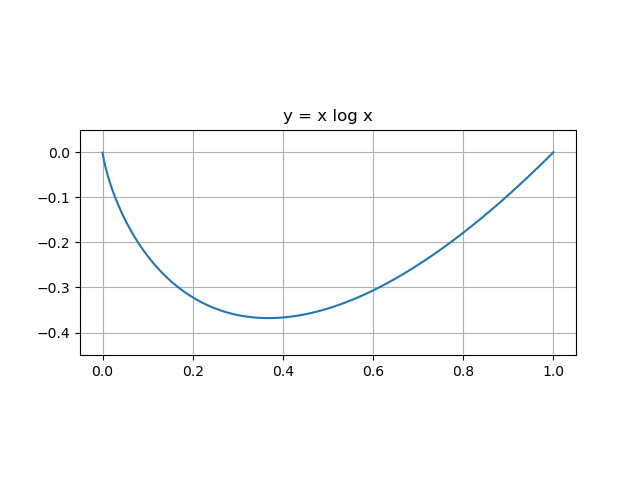
\includegraphics[scale=0.85]{xlogx}
\end{figure}

\newpage
Let $u = -\log x$. Then as $x \to 0^+$, $u \to \infty$.

Also $\df1{\e^u} = \e^{\log x} = x$ so $\df u{\e^u} = -x \log x$. Therefore $$\llim{x \to 0^+} (x \log x) = -\llim{u \to \infty} \f u{\e^u} = -0$$ by Question 2. Therefore $\llim{x \to 0^+} (x \log x) = 0$ as required.

Note that $x^x = \e^{x \log x}$, so $$\llim{x \to 0^+} x^x = \llim{x \to 0^+} \e^{x \log x} = \e^{\,\llim{x \to 0^+} (x \log x)} = \e^0 = 1$$
% }}}

\end{document}
